\documentclass[
	paper = a4,
	10pt,
	english, ngerman,
	oneside,
	numbers=noenddot,
	%parskip	= half, 	% separate paragraphs with half a line
	cdgeometry = symmetric,
	cd = barcolor,
	%chapterpage	= false,
	cdmath = false,
	%slantedgreek=standard,
	captions=tableheading,
	chapteratlists=entry,
	headings=small,
	openany
]{tudscrbook}

\usepackage{tudscrcolor}

\usepackage[utf8]{inputenc}
\usepackage[T1]{fontenc}	

\usepackage{babel}
\usepackage{csquotes}

\usepackage{isodate} 
\usepackage{blindtext}

\usepackage{setspace}
\usepackage{acronym}
\usepackage{scrhack} 	% acronyms result in warning without this
\usepackage{multicol} 	% use multiple columns, used for the acronyms section

\usepackage{enumitem}\setlist{noitemsep} % used for the bullet points in the task section
\usepackage{microtype}	% better spacing

\usepackage{amsmath}
\usepackage{amsfonts}
\usepackage{bm}			% used for making things bold in equations
\usepackage[b]{esvect}

\usepackage{multirow}	% use tables with columns stretching over multiple rows
\usepackage{booktabs}
\setlength\heavyrulewidth{0.25ex}
\usepackage{longtable}

\usepackage[font=footnotesize, format=plain, labelfont=bf]{caption}  % 
\usepackage{subcaption}	% Packages to allow subfigures

\usepackage[bottom, hang, flushmargin]{footmisc}
\renewcommand\hangfootparindent{1em}

%\usepackage{xcolor}
\usepackage{listings}	% Package for displaying code
\definecolor{KeywordBlue}{cmyk}{0.88,0.77,0,0} %88,77,0,0
\definecolor{CommentGreen}{cmyk}{0.87,0.24,1.0,0.13} %87,24,100,13
\lstset{basicstyle=\scriptsize\ttfamily, language=C, commentstyle=\color{CommentGreen}, keywordstyle=\ttfamily\color{KeywordBlue}, backgroundcolor =\color[rgb]{0.95,0.95,0.95}, breaklines=true,literate={\\\%}{{\textcolor{black}{\\\%}}}1}


% some of the metadata for the pdf are defined in the title-file,
% as there are variables like author and title, whích would appear twice otherwise
% hyperref should always be the last package to be loaded
\usepackage[
colorlinks=true,
urlcolor=.,
citecolor=.,
linkcolor=.,        
pdfstartview=FitV,                          		
pdfdisplaydoctitle=true,
hyperfootnotes=false
]{hyperref}
\urlstyle{same}		% use the same font for URLs as for the text

%%% PARAMS %%%
\pdfminorversion=7	% creates pdfs in the version 1.7, which prevents a warning with the logo

% Allow for triple digit page numbers in the toc
%\makeatletter
%\renewcommand*\@pnumwidth{2.1em}
%\renewcommand*\@tocrmarg{3.1em}
%\makeatother

\KOMAoptions{toc=chapterentrydotfill} 	% Add dots in toc for chapters
\setstretch{1.1}						% Adds a bit of space between the lines
\frenchspacing							% Only a single space after a dot


% Parameters to reduce 'Orphans' and 'Widdows'
\clubpenalty 			= 9999
\widowpenalty 			= 9999
\displaywidowpenalty   	= 1602
\brokenpenalty			= 4999	% Parameter for word disjuction on a pagebreak
\pretolerance			= 1100	% Parameter for difference from choosen format
\tolerance 				= 100 	% Parameter for difference from choosen format

% Less coservative parameters for floating objects in LaTeX
% An overview can be found in the book
% The Latex Companions Chapter 6.1
% A good start is
% http://robjhyndman.com/researchtips/latex-floats/

\setcounter{topnumber}{2}
\setcounter{bottomnumber}{2}
\setcounter{totalnumber}{4}
\renewcommand{\topfraction}{0.85}
\renewcommand{\bottomfraction}{0.85}
\renewcommand{\textfraction}{0.15}
\renewcommand{\floatpagefraction}{0.7}
\renewcommand{\textfraction}{0.1}
\setlength{\floatsep}{5pt plus 2pt minus 2pt}
%\setlength{\textfloatsep}{15pt plus 2pt minus 2pt}
%\setlength{\intextsep}{5pt plus 2pt minus 2pt}

\begin{document}

\RedeclareSectionCommand[
  beforeskip=0ex,
  afterskip=0.5ex plus .2ex            
]{chapter}

\frontmatter
\pagenumbering{Roman} 				% needed to capitalize the roman page numbering
\faculty{Fakultät Informatik}
\chair{Professur Softwaretechnologie}
\date{\today}	

\title{Softwaremanagement Beleg}
\author{Richard Voigtmann \matriculationnumber{5075343 Studiengang: Informatik}\and 
	Lara Göschel \matriculationnumber{987654321 Studiengang: Wirtschaftsinformatik}\and 
	Wilhelm Grigoleit \matriculationnumber{456789123 Studiengang: ---} }
\maketitle	
\tableofcontents
\clearpage

\mainmatter
\setcounter{chapter}{0} % sets the number of this chapter to 0

\chapter{Einleitung}
\label{sec:einleitung}
Die zunehmende Digitalisierung im Gesundheitswesen eröffnet vielfältige Möglichkeiten zur Effizienzsteigerung, besseren Informationsbereitstellung und verbesserten Patientenversorgung. In medizinischen Einrichtungen ist jedoch häufig eine heterogene IT-Landschaft vorzufinden, in der Dokumente aus verschiedenen Quellen unstrukturiert abgelegt werden. Daraus resultieren Probleme bei der Informationssuche, Prozessineffizienzen sowie eine eingeschränkte Nachnutzung der Dokumentation. Ziel dieses Projekts ist die Planung eines Entity-Recognition- und -Retrieval-Systems (ER-System) zur Strukturierung und Auffindung medizinischer Informationen in Dokumentensystemen. Der Fokus liegt auf der Integration bestehender Systeme, der Reduktion manueller Suchvorgänge sowie der Einhaltung datenschutzrechtlicher Anforderungen.

{\let\clearpage\relax
\chapter{Stakeholder Interviews}}
\label{sec:stakeholder_interviews}
\section{Vorgehensweise und Zielstellung}
Im Rahmen der Projektplanung wurde eine umfassende Stakeholderanalyse durchgeführt, um die Anforderungen zentraler Interessensgruppen an das geplante Entity-Recognition- und Retrieval-System für medizinische Dokumentensysteme zu identifizieren. Ziel war es, sowohl funktionale als auch nicht-funktionale Anforderungen zu erfassen und dabei die unterschiedlichen Perspektiven aus klinischem Betrieb, technischer Umsetzung und regulatorischem Rahmen zu berücksichtigen.
Die Analyse erfolgte anhand von zwei Interviews mit zentralen Stakeholdergruppen:
\begin{itemize}
	\item Interview 1: mit medizinischem Fachpersonal (Arzt) und Klinikdirektion
	\item Interview 2: mit dem IT-Spezialisten sowie dem Datenschutzbeauftragten der Klinik
\end{itemize}
Die Interviews wurden qualitativ ausgewertet und entlang thematischer Schwerpunkte kategorisiert. Die Ergebnisse flossen direkt in die Anforderungsdefinition und die weitere Projektstrukturierung ein.
\section{Ergebnisse Interview 1: Medizinisches Personal und Klinikdirektion}
\underline{Aktueller Stand und Herausforderungen}
Das medizinische Personal arbeitet täglich mit einer Vielzahl von Dokumenten (z.B. Befunde, Arztbriefe, Laborberichte). Die Informationssuche erfolgt bislang über verschiedene Teilsysteme ohne zentrale Schnittstelle. Dies führt zu ineffizienten Prozessen mit hohem Zeitaufwand (5–20 Klicks pro Abfrage, ca. 100 Zugriffe täglich). Die fragmentierte Systemlandschaft erschwert eine schnelle, kontextbezogene Entscheidungsfindung.
\underline{Anforderungen und Wünsche}
Zentrale Anforderungen sind:
\begin{itemize}
	\item ein kontextsensitives Such- und Dashboardsystem zur automatisierten Darstellung relevanter Informationen
	\item Single Sign-On über alle Subsysteme hinweg
	\item ein modulares, barrierefreies UI mit Unterstützung für Sprachsteuerung
	\item nutzerrollenspezifische Zugriffskonzepte
	\item eine Antwortzeit von unter 3 Sekunden für Standardabfragen
	\item personalisiertes Dashboard mit Speicherung individueller Präferenzen
\end{itemize}
Die Klinikdirektion betont darüber hinaus:
\begin{itemize}
	\item die Effizienzsteigerung als übergeordnetes Ziel zur Entlastung von Personalressourcen
	\item die Einhaltung gesetzlicher Datenschutz- und Interoperabilitätsanforderungen
	\item die Skalierbarkeit des Systems für den klinikweiten Einsatz
	\item die Notwendigkeit frühzeitig testbarer Prototypen und medienwirksamer Präsentationen nach ca. 1,5 Jahren Projektlaufzeit
\end{itemize}
Die Projektumsetzung soll in einem modularen Rollout erfolgen, beginnend mit einem Pilotbetrieb auf einer Station (ca. 100 Patienten).
\section{Ergebnisse Interview 2: IT-Spezialist und Datenschutzbeauftragter}
\underline{Aktueller Stand und Technische Rahmenbedingungen}
Die bestehende IT-Landschaft besteht aus über 40 teilweise proprietären Subsystemen (zentrale Systeme, Sonderanwendungen, Verwaltungswerkzeuge), die auf virtualisierten Maschinen in einem eigenen Rechenzentrum betrieben werden. Es existiert ein ausfallsicheres Backup-System mit redundanter Infrastruktur. Die Nutzung externer Cloud-Services ist untersagt. HL7 und FHIR werden als zentrale Schnittstellenstandards anerkannt.
Der Datenschutzbeauftragte betont die Einhaltung der DSGVO, insbesondere im Hinblick auf Zweckbindung, Datenminimierung und Zugriffsbeschränkung.
\underline{Anforderungen und Wünsche}\\
\underline{Datenschutz und Sicherheit}
\begin{itemize}
	\item Pseudonymisierung und Verschlüsselung sensibler Daten
	\item keine lokale Speicherung personenbezogener Daten auf mobilen Endgeräten
	\item differenzierte Rechtevergabe nach Nutzerrolle (RBAC)
	\item Zwei-Faktor-Authentifizierung (z.B. via TOTP-App)
	\item umfassende Auditierung aller Zugriffe und Aktionen
	\item ausschließliche Verarbeitung innerhalb des geschützten Intranets
	\item Nutzung ausschließlich synthetischer oder pseudonymisierter Snapshots für Tests und Entwicklung
	\item Kein Zugriff auf Live-Daten ohne gesonderte Genehmigung durch ein Datenschutzgremium
\end{itemize}
\underline{Systemintegration und Infrastruktur}
\begin{itemize}
	\item Containerisierter Betrieb (Docker, Kubernetes)
	\item Microservice-Architektur für flexible Skalierbarkeit
	\item Integration in bestehende IT-Umgebung mit abgestimmten Datenformaten und Übergabeprozessen
	\item Kein Caching aufgrund alter Bestandssysteme
	\item Segmentierte Netzwerke, Zugriff IP-basiert
\end{itemize}
\underline{Wartung und Support}
\begin{itemize}
	\item Wartung durch interne IT, mit Unterstützung durch externe Partner bei Entwicklung und Updates (jedoch ohne direkten Infrastrukturzugriff),
	\item dedizierte Update-Fenster (z.B. mittwochs) und ein internes Ticket-System für Fehlerbehandlung,
	\item Entwicklung auf einem separaten, virtuellen Testsystem zur Sicherung des laufenden Betriebs.
\end{itemize}
\underline{Leistungsanforderungen und Skalierung}
\begin{itemize}
	\item Unterstützung von bis zu 50 parallelen Nutzern im Pilotbetrieb, langfristig mehreren Hundert
	\item Antwortzeiten < 3 Sekunden für Standardabfragen
	\item Komplexe Analysen mit akzeptierten Antwortzeiten von wenigen Minuten
	\item Nutzung von Hochleistungssystemen mit dedizierten GPUs
	\item Absicherung kritischer Engpässe durch priorisierte Hardware-Ressourcen
\end{itemize}
\underline{Zeitrahmen}
\begin{itemize}
	\item Projektlaufzeit: 3 Jahre
	\item Nachweis funktionaler Prototypen innerhalb von 1,5 Jahren
	\item Abnahmetest: 3-monatige störungsfreie Betriebsphase zum Projektende
\end{itemize}
\section{Bewertung und Nutzen für das Projekt}
Die Stakeholderinterviews ermöglichten ein tiefes Verständnis der bestehenden Schwachstellen, Prioritäten und Erwartungen. Die Kombination aus medizinischer, technischer und datenschutzrechtlicher Perspektive erlaubt eine differenzierte Anforderungsanalyse.
Die Projektplanung profitiert von einem klar definierten Zielbild eines kontextsensitiven, modularen Systems, das eine nutzerspezifische Anpassbarkeit ermöglicht. Die technische und regulatorische Machbarkeit kann frühzeitig validiert werden, beispielsweise durch den Einsatz synthetischer Daten und die Nutzung der bestehenden internen Infrastruktur. Durch den Abgleich der Anforderungen mit den verfügbaren Ressourcen entsteht eine realistische Roadmap für die Umsetzung. Zudem wird die Kommunikation und Einbindung der Stakeholdergruppen verbessert, etwa durch den Einsatz agiler Sprints, klar definierter Meilensteine und regelmäßiger Abstimmungsgremien. Schließlich werden kritische Erfolgsfaktoren wie Benutzerfreundlichkeit, Datenschutzkonformität und das Antwortzeitverhalten frühzeitig identifiziert und in die Planung integriert.



\let\clearpage\relax
{\chapter{Domainanalyse}
\label{sec:domainanalyse}}
\section{Beschreibung der Domäne}
Die Domäne umfasst klinische Dokumentensysteme, insbesondere die Erfassung, Speicherung, Verarbeitung und Bereitstellung medizinischer Daten innerhalb eines Krankenhauses. Dokumente liegen aktuell in unterschiedlichsten Formaten vor – strukturiert (z.B. HL7-Nachrichten), semi-strukturiert (PDFs, CDA-Dokumente) und unstrukturiert (gescannte Dokumente). Das Zusammenspiel verschiedener Systeme ist mangelhaft, häufig existieren redundante Prozesse und Medienbrüche. Die rechtlichen Rahmenbedingungen sind durch Datenschutzgesetze, Medizinprodukterecht und sektorspezifische IT-Standards geprägt.
\section{Ist-Situation}
Am betrachteten Universitätsklinikum bestehen diverse Insellösungen, die nicht vollständig integriert sind. Informationen sind auf mehrere Systeme verteilt, darunter das KIS, separate Labor- und Entlassungssysteme sowie teilweise analoge Archive. Eine Suche erfordert oft über zehn Klicks und mehrere Logins. Die Informationsaufbereitung ist unzureichend, was zu Verzögerungen in der Patientenversorgung führt. Dokumente im PDF-Format sind nicht durchsuchbar, eine semantische Verknüpfung zwischen verschiedenen Datenquellen existiert nicht.
\section{Zielraum}
Das geplante System soll bestehende Informationssysteme konsolidieren, Datenströme harmonisieren und eine zentrale, durchsuchbare Dokumentenbasis schaffen. Mithilfe von Methoden der natürlichen Sprachverarbeitung und Transfer Learning sollen relevante Entitäten erkannt und in nutzerspezifischen Dashboards visualisiert werden. Die Interaktion mit dem System soll multimodal erfolgen können – über Tastatur, Touch und Sprache. Eine vollständig inhouse betriebene Infrastruktur garantiert die Einhaltung datenschutzrechtlicher Anforderungen. Zudem soll das System HL7- und FHIR-kompatibel sein, um eine künftige Anbindung externer Komponenten zu ermöglichen. Die Domäne unterliegt spezifischen Regularien, darunter die Datenschutz-Grundverordnung (DSGVO), §75c SGB V (IT-Sicherheit im Krankenhaus), die Richtlinie MDR zur Zulassung medizinischer Softwareprodukte sowie der Technische Standard TR-03161 des Bundesamts für Sicherheit in der Informationstechnik (BSI). Technisch kommen etablierte Schnittstellen wie HL7, FHIR und CDA zur Anwendung. Die Einhaltung dieser Normen ist grundlegend für die Zulassung und den sicheren Betrieb des Systems.

{\let\clearpage\relax
\chapter{Zieldefinition}}
\label{sec:zieldefinition}
\section{Projektziel}

Ziel des Projekts ist die Entwicklung einer integrierten Intranet-Plattform zur intelligenten Suche, Kontextanalyse und Visualisierung medizinischer Dokumente und Patienteninformationen. Das geplante System soll verschiedene Subsysteme (KIS, Labor, Medikation, Entlassungsberichte, PDF-Dokumente) semantisch zusammenführen und durch KI-basierte Methoden wie Natural Language Processing (NLP), Transfer Learning und LLMs klinische Entitäten automatisch extrahieren und strukturieren.
Ein personalisiertes Dashboard, eine kontextbasierte Darstellung sowie ein KI-gestützter Assistent sollen den Arbeitsalltag des medizinischen Personals signifikant erleichtern, die Qualität der Datennutzung erhöhen und zur Digitalisierung der klinischen Dokumentation beitragen – unter Einhaltung höchster Datenschutz- und Sicherheitsstandards.
\section{Geschäftsziele}

\begin{center}
\begin{tabular}{|p{5cm}|p{10cm}|}
	\hline
	\textbf{Ziel} & \textbf{Beschreibung} \\
	\hline
	Digitalisierung und Reduktion von Papieraufwand & Nachhaltige Digitalisierung der Dokumentationsprozesse zur Reduktion physischer Archivflächen und Druckkosten. \\
	\hline
	Zukunftssicherheit & Technische und funktionale Skalierbarkeit hinsichtlich Nutzerzahlen, Endgeräte und neuer Datenquellen. \\
	\hline
	Sehr hohe Verfügbarkeit und Ausfallsicherheit & Sicherstellung der Verfügbarkeit auch im Notfall durch redundante Infrastruktur und Ausfallsicherung. \\
	\hline
	Benutzerfreundlichkeit & Klare, konsistente und barrierefreie Oberfläche zur Reduktion der kognitiven Last und Erhöhung der Akzeptanz. \\
	\hline
	Zuverlässige und kontextgerechte Darstellung & Automatisierte Selektion und Visualisierung relevanter Informationen pro Fall. \\
	\hline
	Budgetrahmen und Zeitplan & Einhaltung des Budgets von maximal 500.000€ bei einer Projektlaufzeit von drei Jahren, medienwirksamer Prototyp nach 12–18 Monaten. \\
	\hline
	Gesetzliche Konformität & Einhaltung gesetzlicher Aufbewahrungsfristen (10 Jahre), MDR, DSGVO, BSI TR-03161 und Barrierefreiheitsstandards. \\
	\hline
\end{tabular}
\end{center}



\section{Operative Ziele}
\begin{center}
\begin{tabular}{|p{5cm}|p{10cm}|}
	\hline
	\textbf{Ziel} & \textbf{Beschreibung} \\
	\hline
	Pilotprojekt auf einer Station & Durchführung eines Piloten mit 50 Nutzern und 100 Patienten zur Evaluation im Echtbetrieb. \\
	\hline
	Antwortzeiten unter 3 Sekunden & Schnelle Entscheidungsprozesse durch kurze Antwortzeiten bei Standardabfragen. \\
	\hline
	Weniger als 10 Klicks pro Informationsabruf & Deutliche Reduktion der Interaktionslast im Vergleich zum Ist-Zustand. \\
	\hline
	Zentraler Login mit Langzeit-Authentifizierung & Single Sign-On (SSO) mit Zwei-Faktor-Authentifizierung zur Erhöhung von Sicherheit und Benutzerfreundlichkeit. \\
	\hline
	Interne Datenverarbeitung & Ausschließliche Verarbeitung im gesicherten Intranet, kein Cloudzugriff oder Datenexport. \\
	\hline
	Kompatibilität mit Bestandssystemen & Ergänzung bestehender KIS-Komponenten ohne deren vollständige Ablösung. \\
	\hline
\end{tabular}
\end{center}


\section{Stakeholderziele}
\begin{center}
\begin{tabular}{|p{4cm}|p{5cm}|p{6cm}|}
	\hline
	\textbf{Stakeholder} & \textbf{Ziel} & \textbf{Beschreibung} \\
	\hline
	Medizinisches Personal & Zeitersparnis und Effizienz & Reduzierte Klicks, zentrale Suche und kontextbezogene Darstellung ermöglichen eine spürbare Zeitersparnis. \\
	
	& Intuitive Bedienung & Bedienbarkeit ohne umfassende Schulungen, anpassbare Dashboards entsprechend individueller Arbeitsstile. \\
	
	& Sprachsteuerung & Sprachbasierte Interaktion für hygienisch sensible Situationen, z.B. bei Visiten oder Operationen. \\
	
	& KI-gestützte Unterstützung & Ad-hoc-Suche in natürlicher Sprache, semantische Abfragen und Anomalieerkennung zur Unterstützung medizinischer Entscheidungen. \\
	\hline
	Klinikdirektion & Hohe Verfügbarkeit und Sicherheit & Ausfallsicherheit, Rechtemanagement mit Zwei-Faktor-Authentifizierung und differenzierter Rollensteuerung. \\
	
	 & Backup und Kostenkontrolle & Nutzung der vorhandenen Serverarchitektur für Backup und Recovery, Kostenkontrolle durch Meilensteine und Evaluationsphasen. \\
	
	 & Langfristige Skalierbarkeit & Sicherstellung von Skalierbarkeit und Wartbarkeit für den Klinikbetrieb. \\
	\hline
\end{tabular}
\end{center}


\section{Ergebnisziele}
\begin{center}
\begin{tabular}{|p{5cm}|p{10cm}|}
	\hline
	\textbf{Ergebnisziel} & \textbf{Messkriterium} \\
	\hline
	Antwortzeiten & Standardabfragen unter 3 Sekunden \\
	\hline
	Interaktionen pro Suche & Weniger als 10 Interaktionen \\
	\hline
	Zeitersparnis & Mindestens 30\% im Klinikalltag \\
	\hline
	Nutzerzufriedenheit & Mindestens 75\% positives Feedback im Pilottest \\
	\hline
	Prototyp und Pilot & Funktionaler Prototyp nach 6 Monaten, Pilotbetrieb nach spätestens 12 Monaten \\
	\hline
\end{tabular}
\end{center}


\section{Nicht-Ziele}
\begin{center}
	\begin{tabular}{|p{5cm}|p{10cm}|}
		\hline
		\textbf{Was nicht erreicht werden soll} & \textbf{Begründung} \\
		\hline
		Vollständiger Ersatz des KIS & Das bestehende KIS bleibt Hauptsystem für Patientenstammdaten und Behandlungsdokumentation. \\
		\hline
		Mobile Speicherung personenbezogener Daten & Schutz vor Datenverlust bei Geräteverlust. \\
		\hline
		Integration externer Mandanten im Pilotbetrieb & Fokussierung auf interne Pilotstation. \\
		\hline
		Komplette Neugestaltung der UI & Wahrung der Vertrautheit und Akzeptanz der Nutzer. \\
		\hline
		Automatisierte Entscheidungsfindung & Das System unterstützt, ersetzt aber keine klinische Verantwortung. \\
		\hline
		Autorisierte Löschung kritischer Daten & Vermeidung von Sicherheits- und Compliance-Risiken. \\
		\hline
	\end{tabular}
\end{center}
{\let\clearpage\relax
\chapter{Technologieevaluation}}
\label{sec:technologieevaluation}
6 Technologieevaluation und Konkurrenzanalyse
\section{Ziel und Vorgehen}
Ziel dieses Arbeitspakets war es, den aktuellen Stand der Technologieentwicklung im Bereich medizinischer Dokumentenverarbeitung zu analysieren, geeignete technische Komponenten für die geplante Entity-Recognition- und Retrieval-Plattform auszuwählen und die Lösung strategisch gegenüber bestehenden Markt- und Speziallösungen zu positionieren.\\
\underline{Das Vorgehen erfolgte in vier Schritten:}
\begin{enumerate}
	\item \textbf{Anforderungsdefinition:} Ableitung funktionaler und nicht-funktionaler Anforderungen aus Stakeholderinterviews und den Projektzielen (z.B. HL7/FHIR-Unterstützung, kontextsensitive Suche, Barrierefreiheit, Datenschutz)
	\item \textbf{Marktanalyse (State of the Art):} Untersuchung bestehender Systeme in den Bereichen Datenvirtualisierung, Business Intelligence (BI) und medizinische Visualisierung
	\item \textbf{Technologieevaluation:} Bewertung geeigneter Technologien mittels Scoring-Modell nach Funktionsumfang, Standardkonformität, Integrationsfähigkeit, Stabilität, Community-Support und Eignung für den klinischen Kontext
	\item \textbf{Konkurrenzanalyse:} Vergleich mit führenden Marktakteuren anhand eines Kiviat-Diagramms und einer SWOT-Analyse zur strategischen Positionierung
\end{enumerate}

\chapter{Konkurrenzanalyse}
\label{sec:konkurrenzanalyse}
{\let\clearpage\relax
\chapter{Ablauforganisation}}
\label{sec:ablauforganisation}

\section{Einsatz des Spiralmodells}
Im Projekt zur Entwicklung eines Datenaufbereitungssystems für ein Krankenhaus kommt das Spiralmodell zum Einsatz, um iterative Entwicklung und systematisches Risikomanagement miteinander zu verbinden. Aufgrund der langen Laufzeit, der hohen Komplexität sowie ethischer und datenschutzrechtlicher Anforderungen eignet sich dieses Vorgehensmodell besonders.

\begin{figure}[ht]
  \centering
  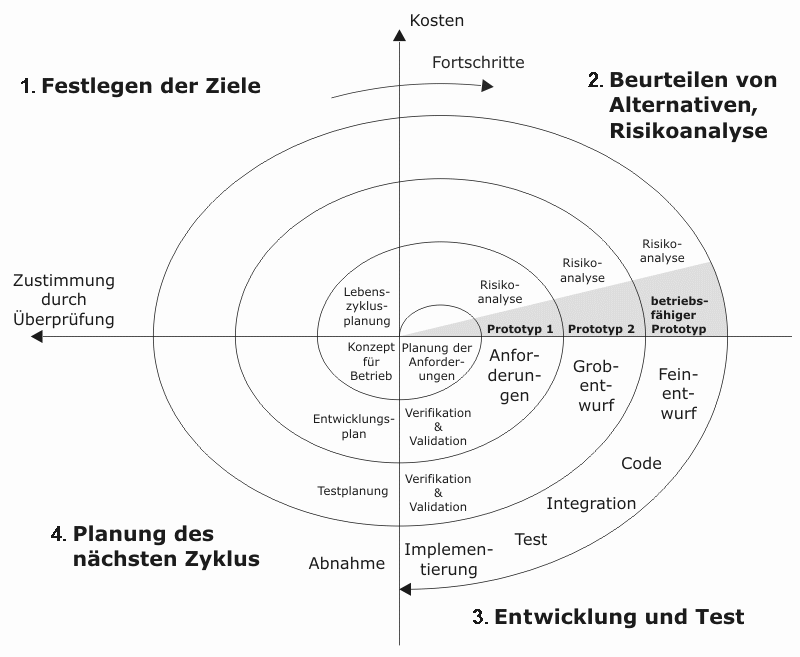
\includegraphics[width=0.6\textwidth]{fig/Spiralmodel_nach_Boehm.png}
  \caption{Das Spiralmodell im Projektkontext}
\end{figure}

\section{Umsetzung Teams und Kommunikation}
Die Umsetzung erfolgt durch zwei parallel arbeitende Teams: eines für die Benutzeroberfläche (UI) und eines für die Datenverarbeitung (Data). Beide Teams arbeiten eigenständig in jeweils eigenen Spiralzyklen. Die Kommunikation erfolgt über definierte Schnittstellen und wird durch die Teamleiter koordiniert. Fachliche Fragen stimmen die Teams bei Bedarf mit IT, ärztlichem Personal, Klinikleitung und Datenschutzbeauftragten ab. Die Infrastrukturverantwortung liegt beim Data-Team, juristische Fragestellungen werden durch interne oder externe Juristen begleitet.

% Bildvorschlag: Kommunikationsstruktur aus Folie 6 oder 7
\begin{figure}[ht]
  \centering
  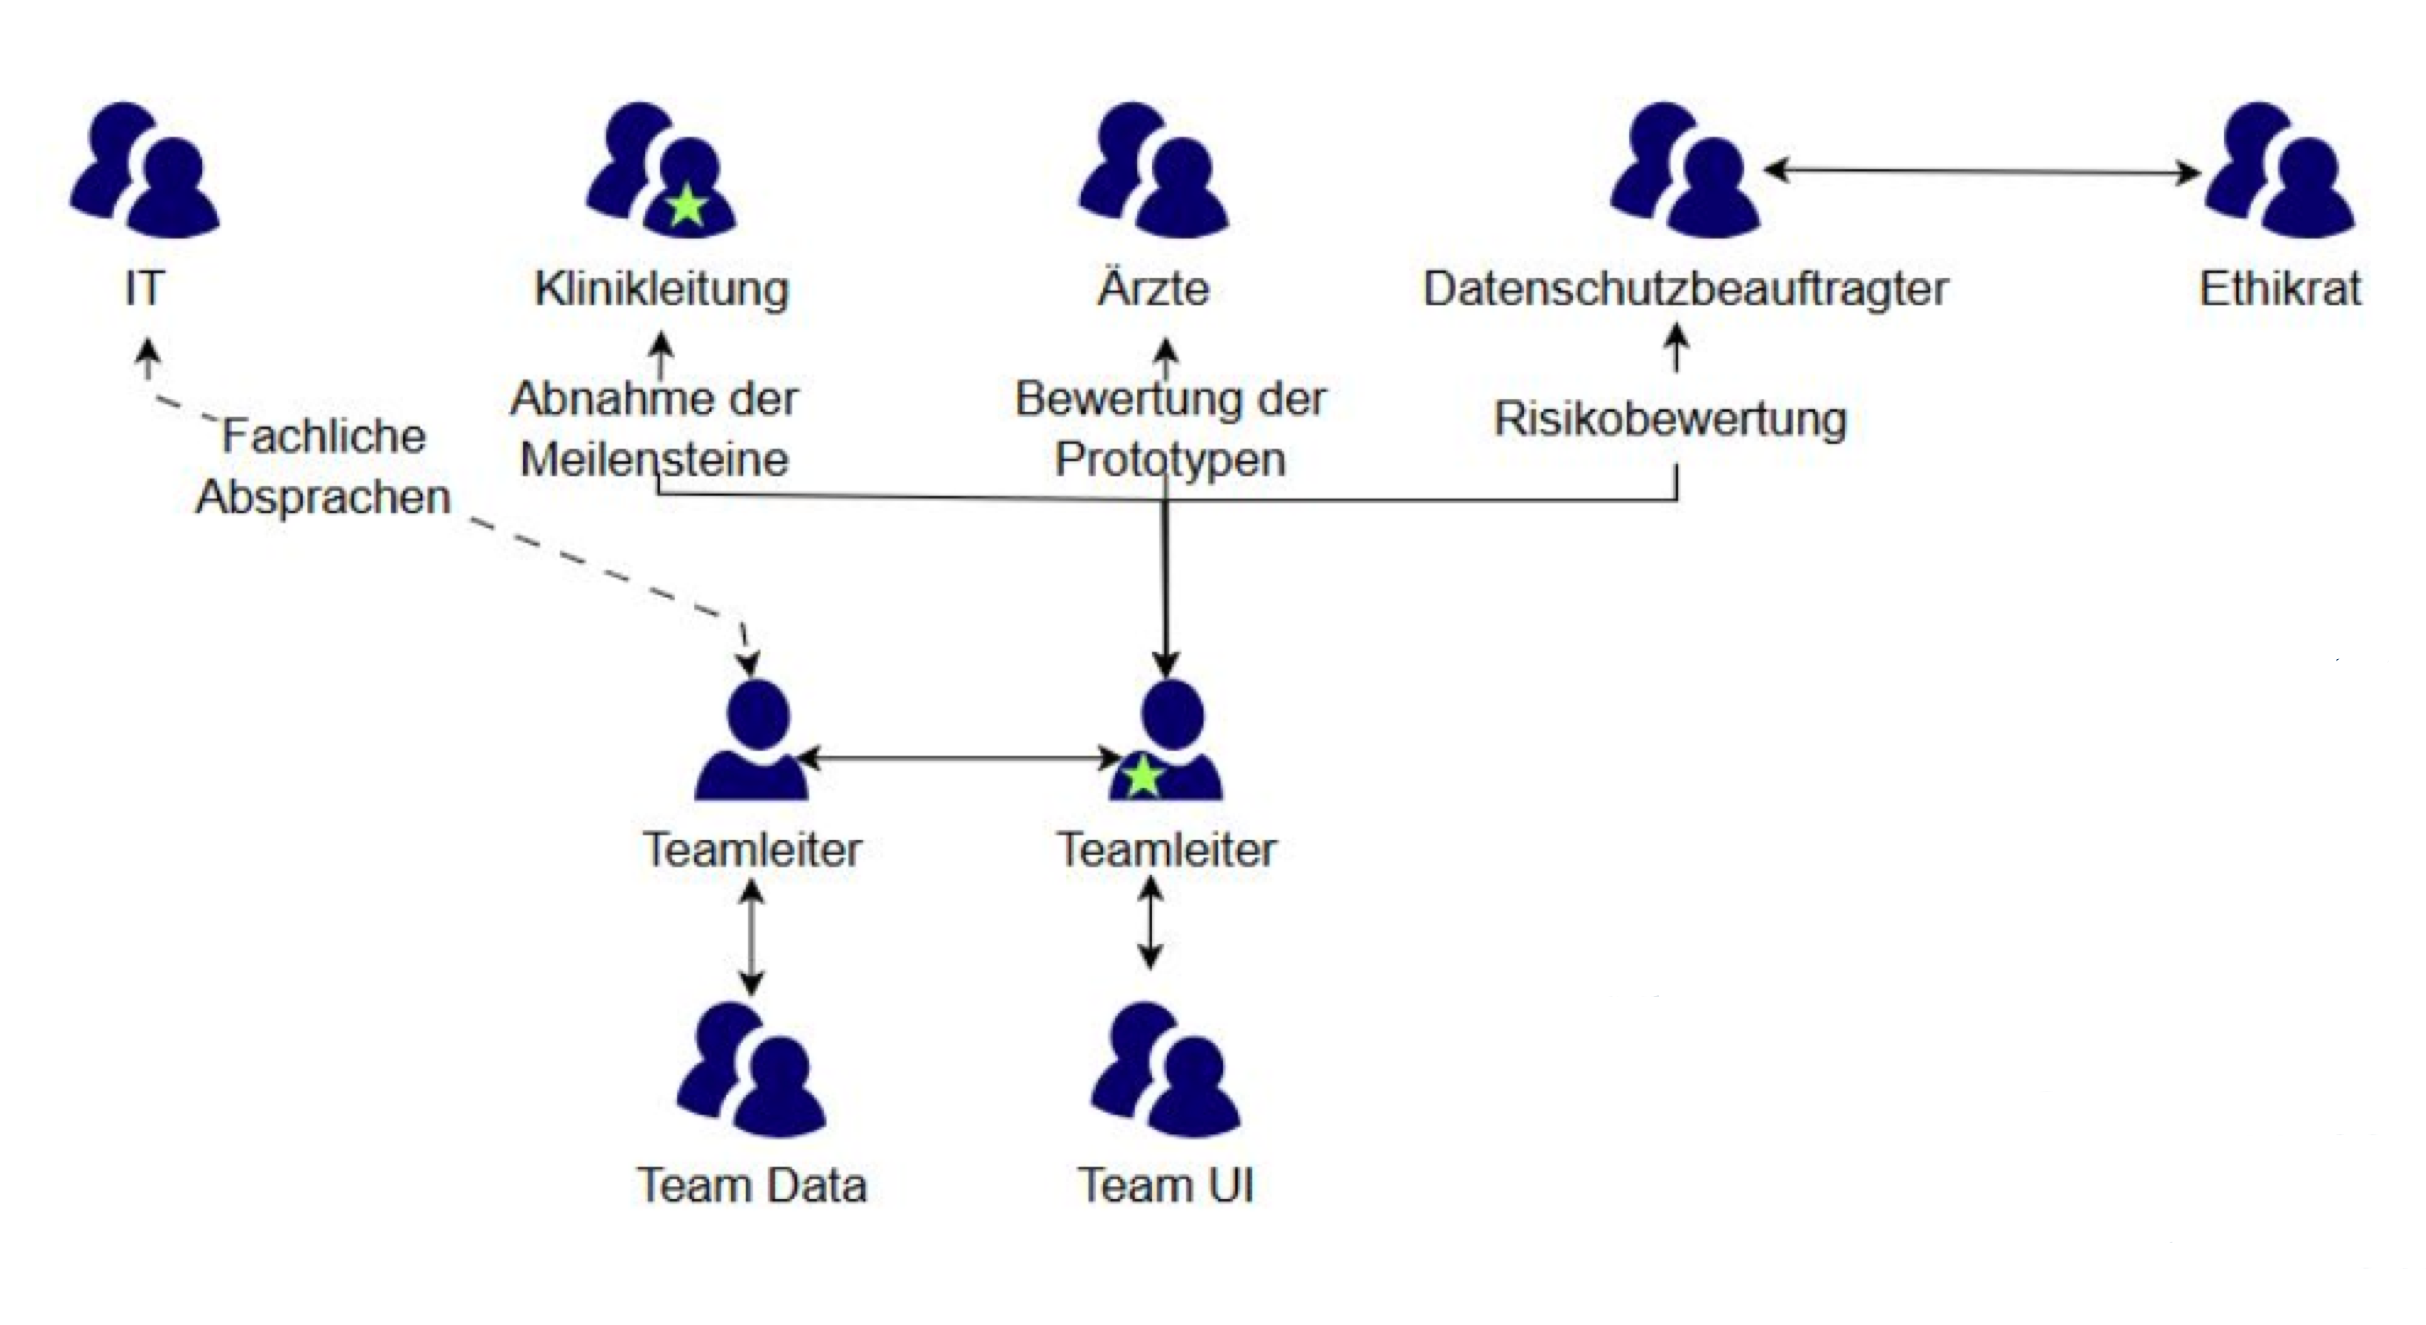
\includegraphics[width=0.8\textwidth]{fig/kommunikation.png}
  \caption{Kommunikationsstruktur der Projektteams}
\end{figure}

\section{Spiralzyklen}
Der Ablauf gliedert sich in mehrere Spiralzyklen mit jeweils definierten Zielen, Risikoanalysen, Entwicklungsmaßnahmen und Evaluationen:

\textbf{Durchlauf 0 – Projektplanung:} In dieser Phase erfolgt die Bedarfsanalyse, die Zieldefinition, eine Technologie-Evaluation sowie die Kosten- und Zeitplanung. Die Projektstruktur wird festgelegt, Interviews mit relevanten Stakeholdern werden geführt und die juristische Prüfung schließt den Durchlauf ab.

% Bildvorschlag: Ablaufplan aus Folie 8
\begin{figure}[ht]
  \centering
  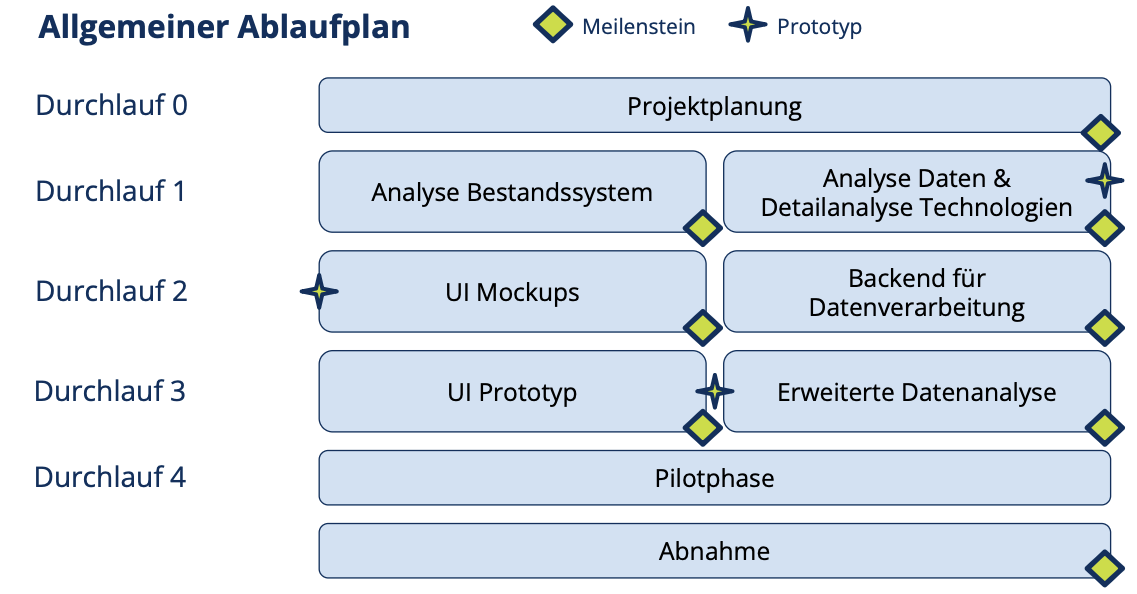
\includegraphics[width=\textwidth]{fig/ablaufplan.png}
  \caption{Übersicht über die Spiralzyklen}
\end{figure}

\textbf{Durchlauf 1 – Analyse des Bestandssystems:} Das UI-Team analysiert reale Nutzungsszenarien und dokumentiert typische Workflows gemeinsam mit medizinischem Personal. Gleichzeitig bewertet das Data-Team verfügbare Technologien hinsichtlich Datenschutz, Kompatibilität und Funktionalität.

\textbf{Durchlauf 2 – Mockup und Backend:} Das UI-Team erstellt klickbare Mockups auf Basis synthetischer Daten und bewertet sie anhand von Effizienzkriterien wie Klickanzahl und Nutzerfeedback. Das Data-Team entwickelt erste Scraper sowie ein zentrales Backend zur normgerechten Aggregation und Speicherung der Daten.

\textbf{Durchlauf 3 – Funktionale Prototypen:} Das UI-Team entwickelt ein interaktives Dashboard mit rollenbasiertem Zugriff, mobiler Unterstützung, Barrierefreiheit und KI-gestützter Datenverarbeitung. Funktionen wie ein „ChatGPT“-ähnliches Interface und eine Anomalieerkennung kommen zum Einsatz. Parallel entwickelt das Data-Team ein Language Model zur erweiterten Analyse und Korrelation der Daten.

\textbf{Durchlauf 4 – Pilotphase und Abnahme:} Das Gesamtsystem wird in einer Pilotumgebung konfiguriert und unter Echtbedingungen getestet. Monitoring, Nutzerschulung und eine normenkonforme Prüfung durch IT, ärztliches Personal, Projektleitung und Datenschutzbeauftragte bilden die Grundlage für die finale Abnahme.


Während aller Spiralzyklen erfolgt eine kontinuierliche Risikobewertung. Besondere Aufmerksamkeit gilt dabei der Datensicherheit, der Integration von KI-Komponenten sowie der Systemkompatibilität. Der Ethikrat ist stets eingebunden, sobald nicht-synthetische Daten oder automatisierte Entscheidungsprozesse ins Spiel kommen. Für KI-Komponenten werden ISO/IEC-Normen beachtet. Die Evaluation des UI basiert unter anderem auf Nutzerfeedback über Systeme wie den SUS oder den UEQ.

{\let\clearpage\relax
\chapter{Produktplanung}}
\label{sec:produktplanung}

\section{Zielsetzung und Systemverständnis}
Ziel der Produktplanung war es, ein System zur kontextsensitiven Entitätenerkennung und zum Dokumentenretrieval für medizinische Einrichtungen zu entwerfen. Der Fokus lag auf der Entwicklung eines Prototyps, der in eine bestehende Infrastruktur einer Pilotstation integriert werden kann. Dabei wurde besonderer Wert auf die Einhaltung medizinischer Standards, die Zeitersparnis im Klinikalltag und die Nutzerfreundlichkeit gelegt.

\section{Strukturierte Produktplanung}
Diese drei Ebenen wurden innerhalb eines sechsstufigen Planungsprozesses erstellt:
\vspace{-\topsep}
\begin{enumerate}
	\item Systemverständnis und Zielanalyse
	\item Erstellung des Produktstrukturplans (PBS)
	\item Erstellung des Artefaktstrukturplans (ABS)
	\item Erstellung des Arbeitsstrukturplans (WBS)
	\item Konsistenzprüfung mittels Kreuzmatrix
	\item Formulierung der Produktvision
\end{enumerate}

\subsection{Produktstrukturplan (PBS)}

Der Produktstrukturplan identifiziert die zentralen Bestandteile des geplanten Systems. Das Gesamtsystem wurde als integriertes Informations- und Managementsystem für medizinische Umgebungen konzipiert.\\
Die Hauptkomponenten sind in der zweiten Ebene des PBS.
\begin{figure}[ht]
	\centering
	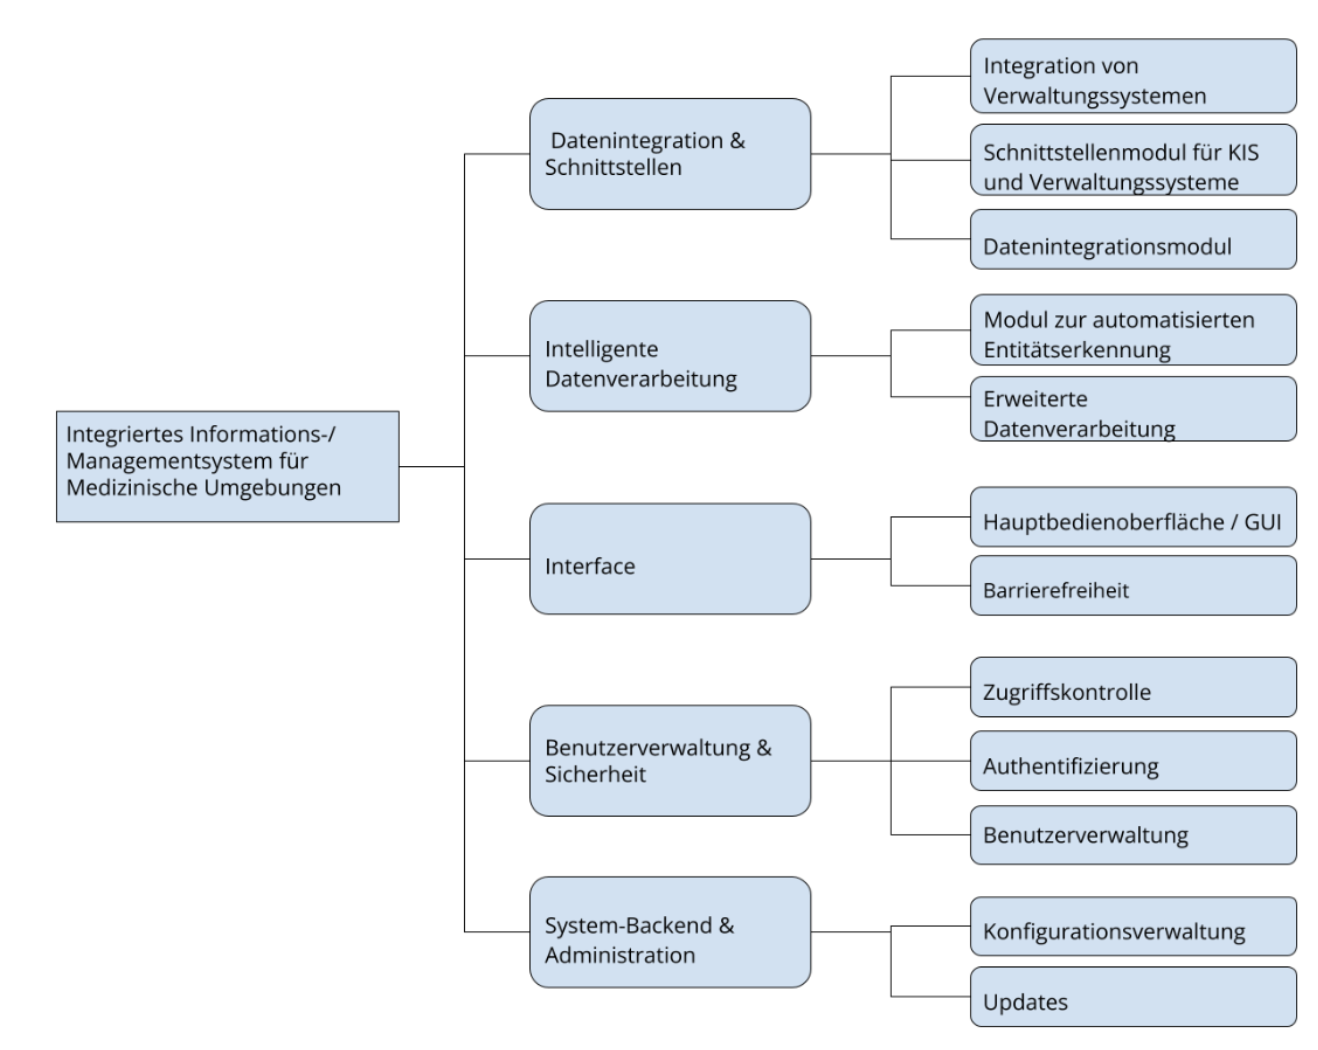
\includegraphics[width=1\textwidth]{fig/planung_alle_ebenen.png}
	\caption{Produktstrukturplan (PBS) des geplanten Systems}
	\label{fig:produktstrukturplan}
\end{figure}
\\
Jede dieser Komponenten wurde weiter in Teilfunktionen und Module gegliedert, ohne zeitliche Abfolge, sondern mit dem Fokus auf die Zielstruktur des Endprodukts.

\pagebreak
\subsection{Artefaktstrukturplan (ABS)}
\begin{figure}[ht]
	\centering
	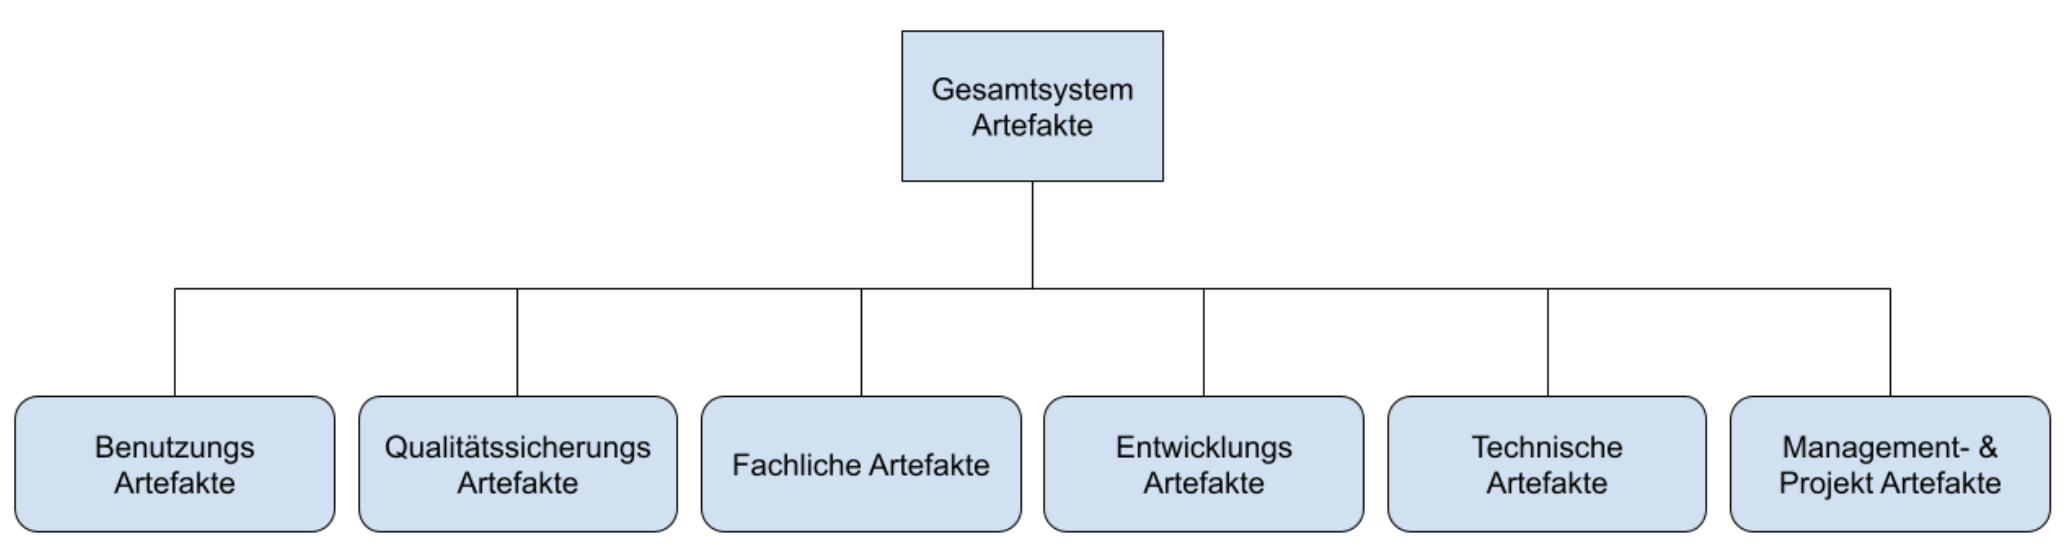
\includegraphics[width=1\textwidth]{fig/abs.png}
	\caption{Artefaktstrukturplan (ABS)}
	\label{fig:artefaktstrukturplan}
\end{figure}
Der Artefaktstrukturplan benennt die fachlichen, technischen, entwicklungsbezogenen, qualitativen und organisatorischen Artefakte, die im Entwicklungsverlauf entstehen. \\
Dazu gehören unter anderem:
\begin{itemize}
	\item Anforderungsspezifikation, Stakeholderanalyse und Sicherheitsanforderungen
	\item Architekturdiagramme, Schnittstellenspezifikationen
	\item Annotierte Trainingsdaten, Code-Repositories, GUI-Prototypen
	\item Testkonzepte, Testergebnisse, Fehlermanagement
	\item Benutzer- und Administrationshandbücher
	\item Projektstrukturplan, Risikomatrix, Statusberichte
\end{itemize}

\subsection{Arbeitsstrukturplan (WBS)}
\begin{figure}[ht]
	\centering
	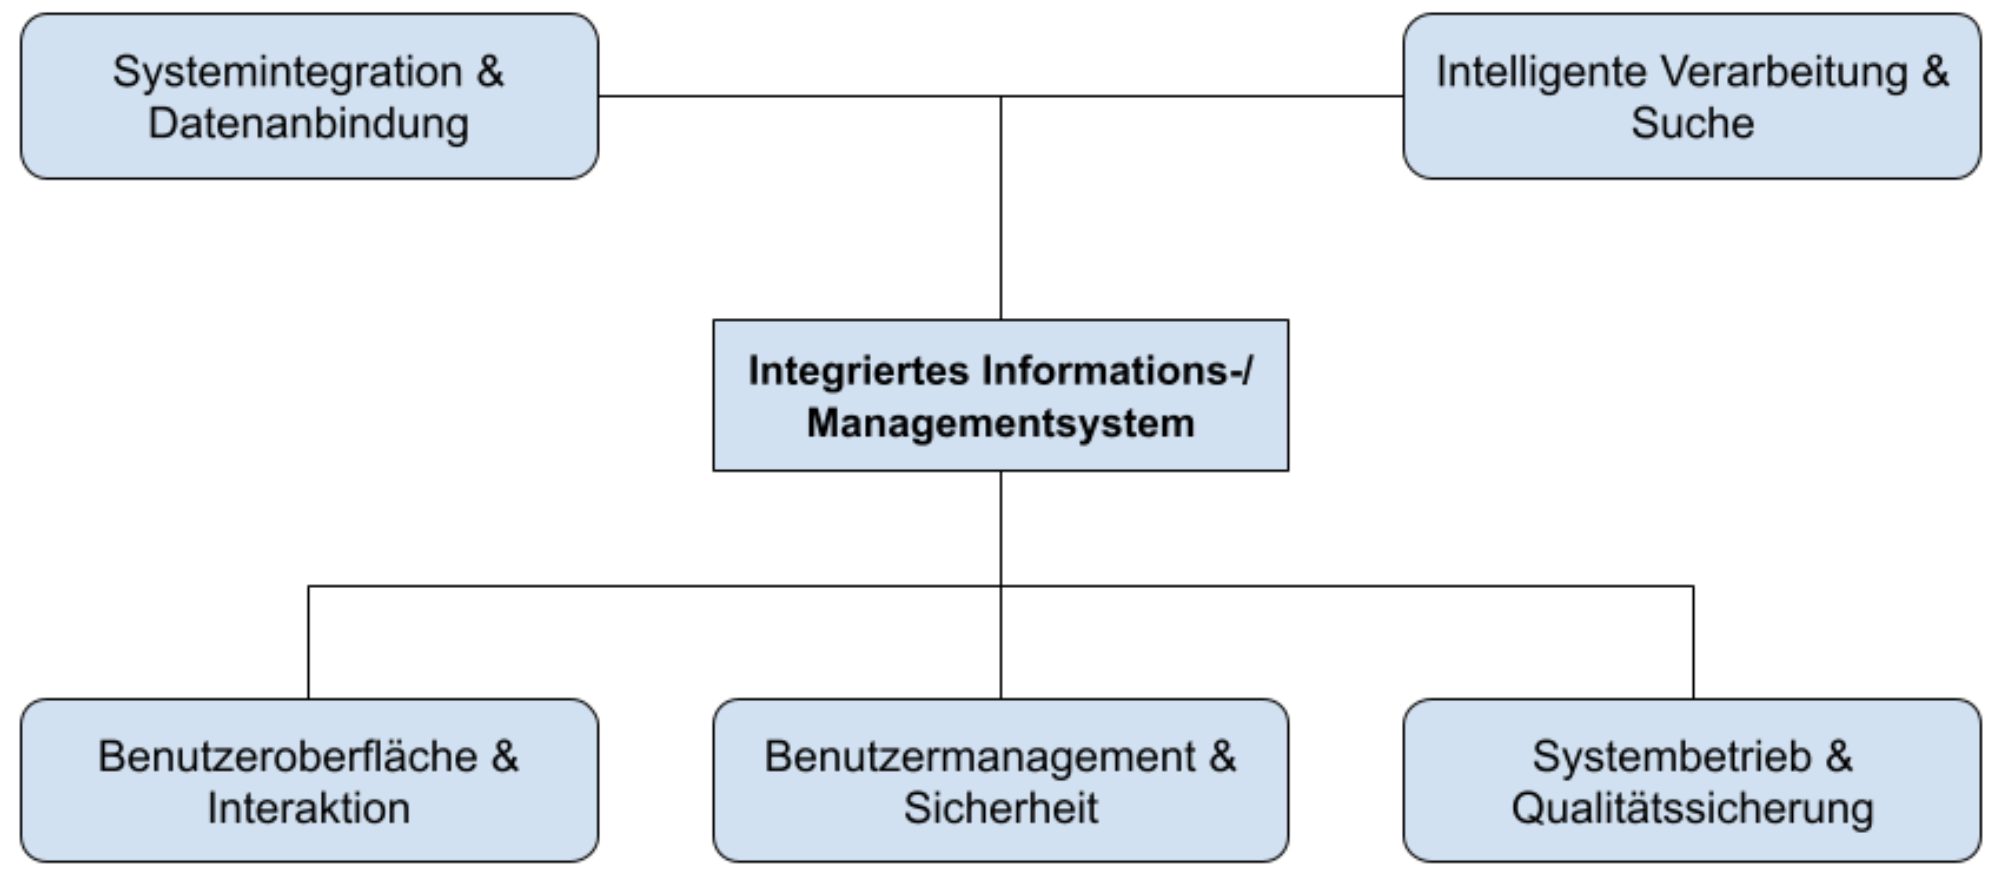
\includegraphics[width=1\textwidth]{fig/wbs.png}
	\caption{Arbeitsstrukturplan (WBS)}
	\label{fig:arbeitsstrukturplan}
\end{figure}
Der Arbeitsstrukturplan unterteilt das Projekt in konkrete Arbeitspakete (AP). Diese Pakete enthalten Angaben zu Inhalten, Zielen, Aufwand, Ressourcenbedarf und Abhängigkeiten. Beispiele sind:
\begin{itemize}
	\item \textbf{AP 1:} API-Integration für Verwaltungssysteme
	\item \textbf{AP 5:} Entwicklung eines NLP-Moduls zur medizinischen Entitätenerkennung
	\item \textbf{AP 9:} Authentifizierung und Zugriffskontrolle (inkl. SSO und 2FA)
\end{itemize}
Jedes Arbeitspaket wurde mit Leistungsfortschrittsindikatoren, geschätztem Aufwand in Personenstunden sowie Kosten versehen.

\subsection{Konsistenzprüfung}
\begin{figure}[ht]
	\centering
	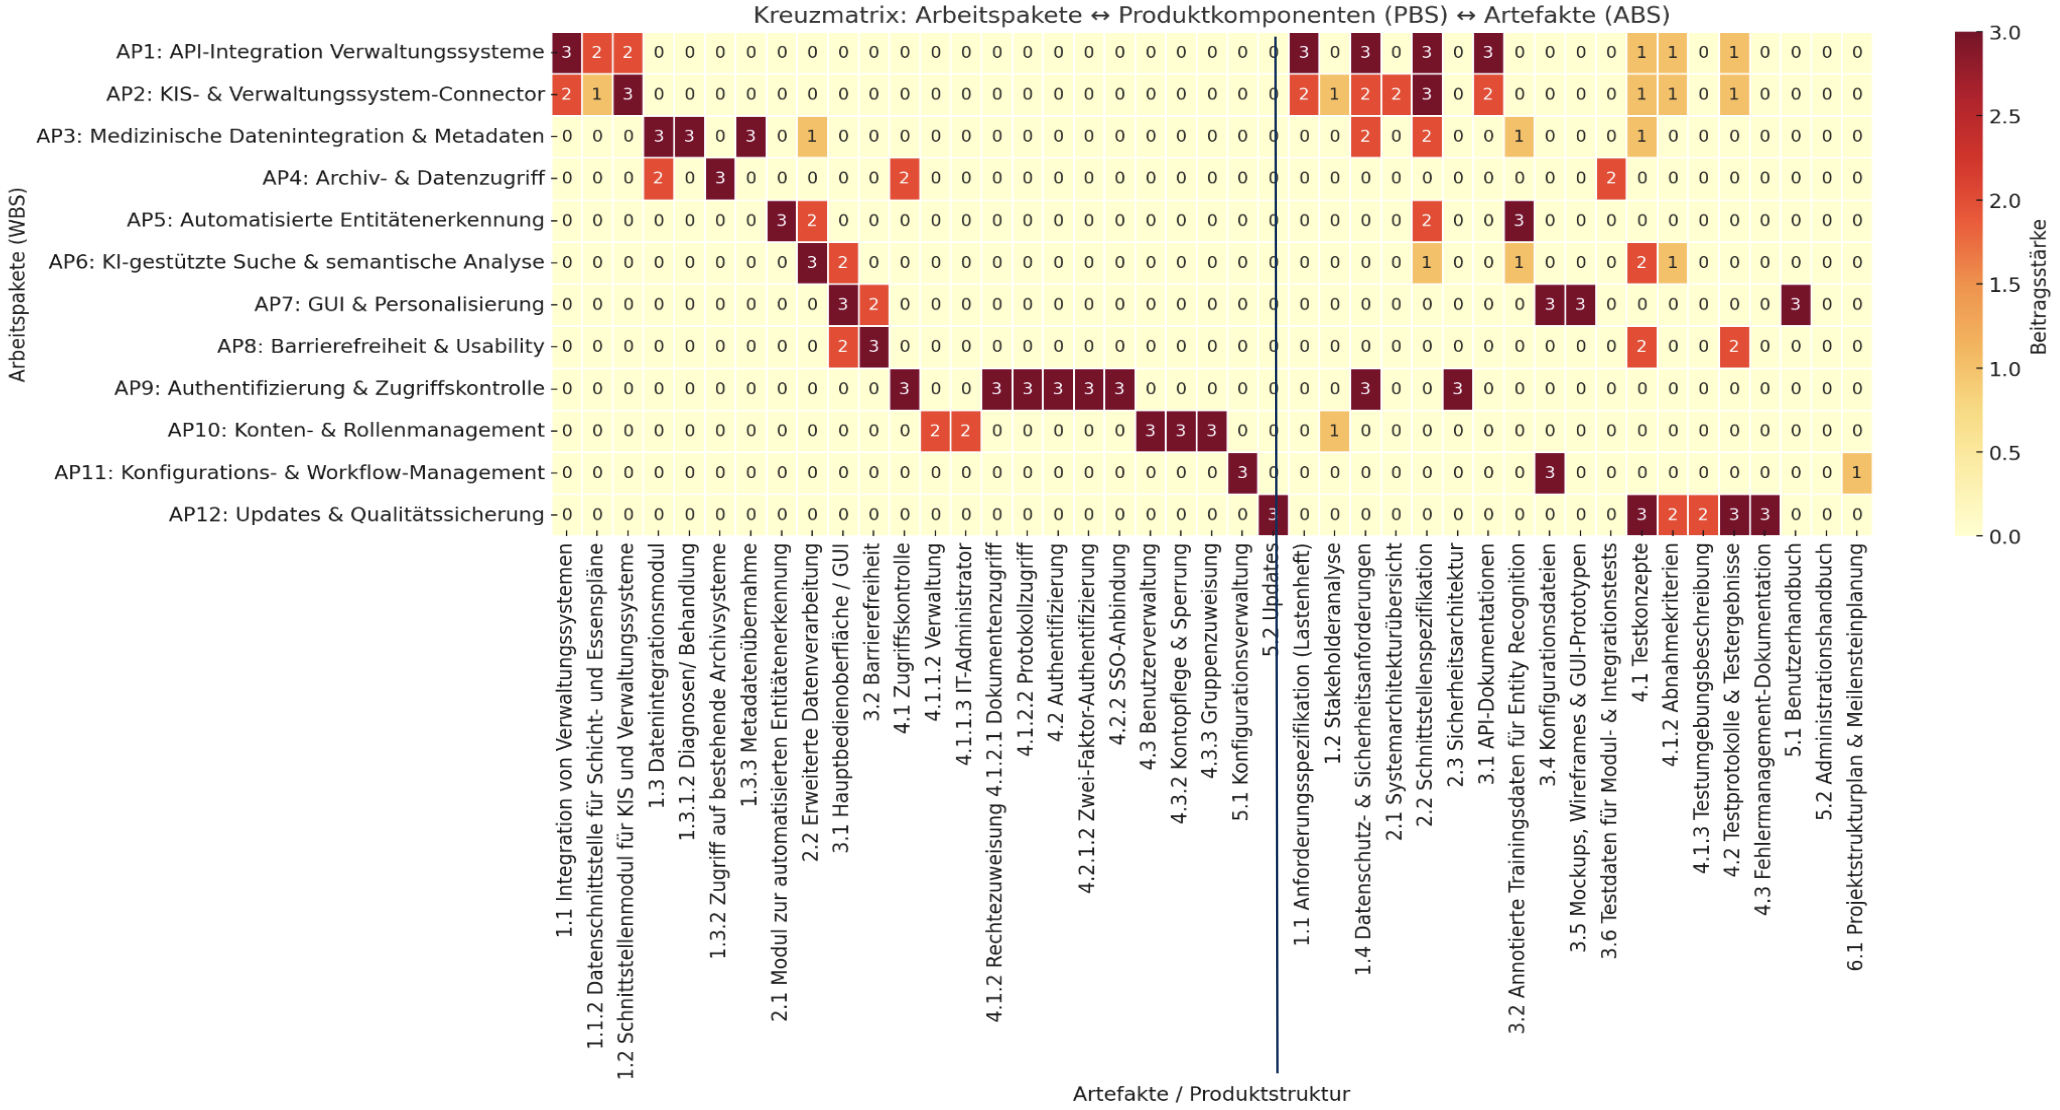
\includegraphics[width=1\textwidth]{fig/kreuzmatrix.png}
	\caption{Kreuzmatrix zur Konsistenzprüfung}
	\label{fig:kreuzmatrix}
\end{figure}
Im letzten Schritt wurde eine Kreuzmatrix verwendet, um die Konsistenz zwischen PBS, ABS und WBS zu prüfen. So konnten Lücken oder Inkonsistenzen frühzeitig identifiziert und behoben werden.

%\section{Fazit}
%Die durchgeführte Produktplanung bietet eine solide Basis für die weitere Projektumsetzung. Sie ermöglicht eine klare Ressourcenallokation, eine strukturierte Zeitplanung sowie die Definition von Teststrategien und Risikomanagementmaßnahmen. Besonders hervorgehoben wurden die Bereiche Datenintegration und Benutzerverwaltung, da sie zentrale Herausforderungen im Klinikalltag adressieren.


{\let\clearpage\relax
\chapter{Arbeitsplanung}}
\label{sec:ablaufplanung}

\section{Vorgangsliste und Abhängigkeiten}
Zur Ablaufplanung wird eine \textbf{Vorgangsliste} mit 12 Arbeitspaketen erstellt. Diese diente als Grundlage für:
\begin{itemize}
  \item Identifikation von Abhängigkeiten,
  \item Schätzung von Dauern und Zeitpunkten,
  \item Zuordnung von Ressourcen.
\end{itemize}

Die Abhängigkeiten zwischen Arbeitspaketen werden durch Einschätzung und Erfahrung identifiziert. Es ergeben sich sowohl \textbf{stringente} als auch \textbf{parallele Abläufe.}

Die Aufwandsschätzung erfolgte mithilfe der \textbf{gewichteten Drei-Punkt-Schätzung}:
\[
A = \frac{A_o + 2 \cdot A_w + A_p}{4}
\]
Dabei stehen $A_o$, $A_w$ und $A_p$ für den optimistischen, wahrscheinlichsten und pessimistischen Aufwand.

\begin{figure}[ht]
	\centering
	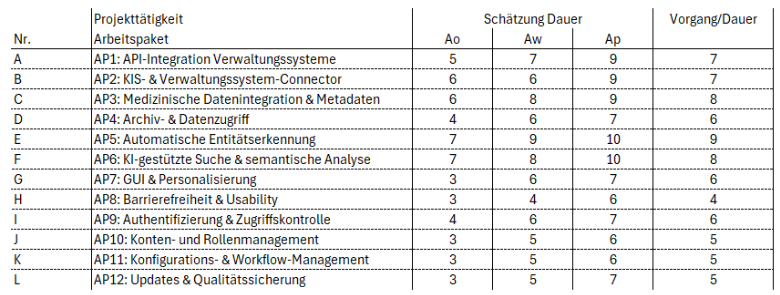
\includegraphics[width=0.9\textwidth]{fig/vorrangliste.png}
	\caption{Vorrangliste}
	\label{fig:vorrangliste}
\end{figure}

\section{Netzpläne und Zeitberechnungen}
Basierend auf der Vorgangsliste werden \textbf{Netzpläne} erstellt, um zeitliche Abläufe zu berechnen. Dabei kamen zwei Verfahren zum Einsatz:

\subsection{Vorwärtsrechnung}
\begin{itemize}
  \item Frühester Anfang ($FA$) beginnt bei 0 bei Startpaketen.
  \item Frühestes Ende: $FE = FA + \text{Dauer}$.
  \item Für Folgepakete: $FA = \max(FE_{\text{Vorgänger}})$.
\end{itemize}

\subsection{Rückwärtsrechnung}
\begin{itemize}
  \item Spätestes Ende ($SE$) des Endpakets entspricht dem $FE$.
  \item Spätester Anfang: $SA = SE - \text{Dauer}$.
  \item Für Vorgänger: $SE = \min(SA_{\text{Nachfolger}})$.
\end{itemize}

\begin{figure}[ht]
	\centering
	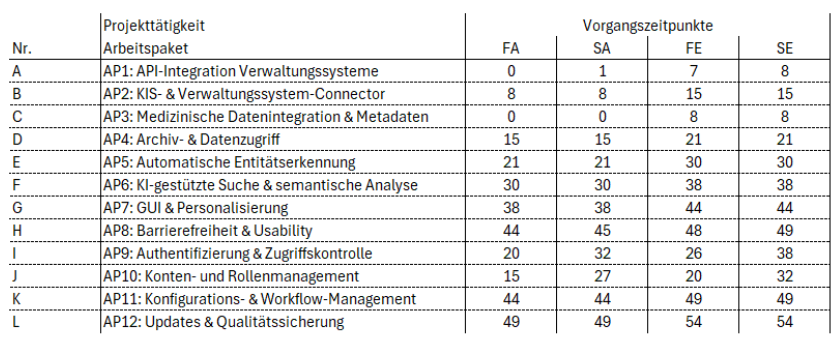
\includegraphics[width=0.9\textwidth]{fig/vorrangliste2.png}
	\caption{Vorrangzeitpunkte}
	\label{fig:vorrangzeitpunkte}
\end{figure}

\subsection{Pufferzeiten}
Pufferzeit beschreibt den Zeitrahmen, in dem ein Arbeitspaket ohne Projektverzögerung verschoben werden kann:
\[
Puffer = SE - FE = SA - FA
\]

\textbf{Beispiel:} Für AP10 ergibt sich ein Puffer von $32 - 20 = 27 - 15 = 12$.

\subsection{Kritische Aktivitäten}
Im Netzplan werden \textbf{kritische Pfade} identifiziert. Diese Arbeitspakete besitzen keinen Puffer und dürfen nicht verzögert werden, da sie direkt das Projektende beeinflussen. Der \textbf{kritische Pfad} wird rot markiert.

\subsection{Umrechnung in Wochendauer}
\begin{itemize}
	\item Gesamtprojektdauer: $3 Jahre = 36 Monate = 156 Wochen$
	\item Gesamtaufwand des kritischen Pfads: 57 Einheiten (inkl. AP13 - Dokumentation \& Schulung)
	\item Dauer des kritischen Pfads = 57 2,74 = 156,18 Wochen
\end{itemize}
\[
	\frac{156 Wochen}{57 Aufwand} \approx 2,74 \frac{Wochen}{Aufwand}
\]
\begin{figure}[ht]
	\centering
	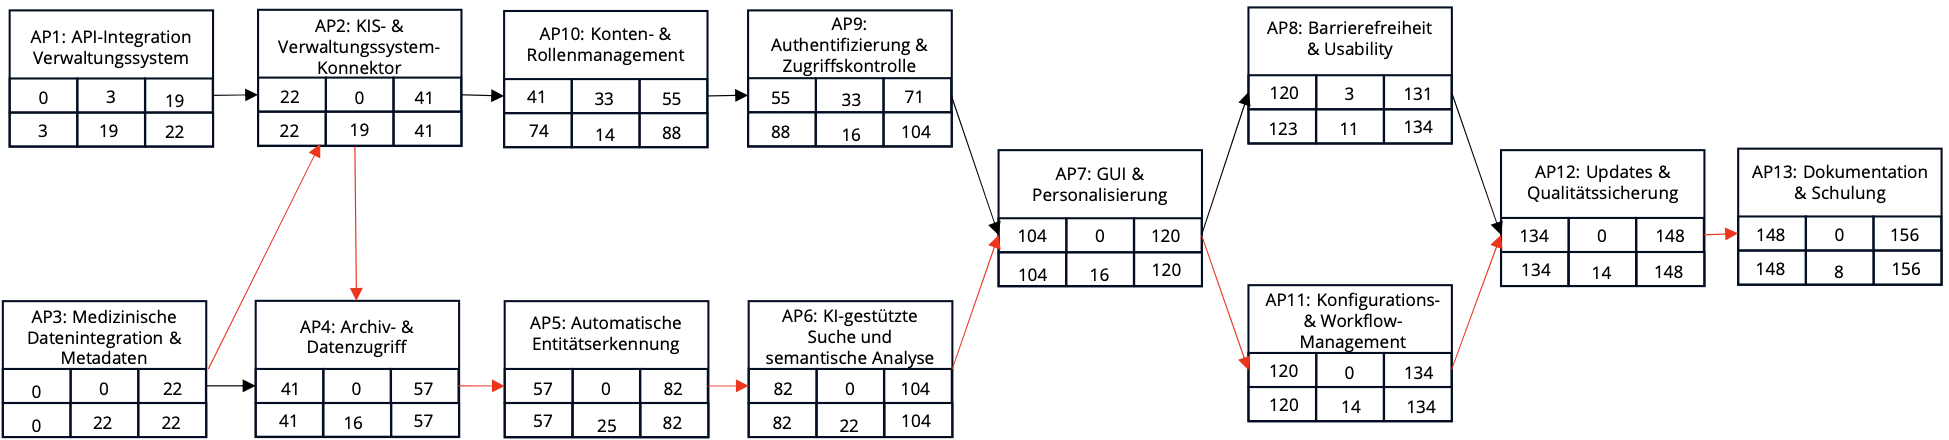
\includegraphics[width=1\textwidth]{fig/Netzplan.png}
	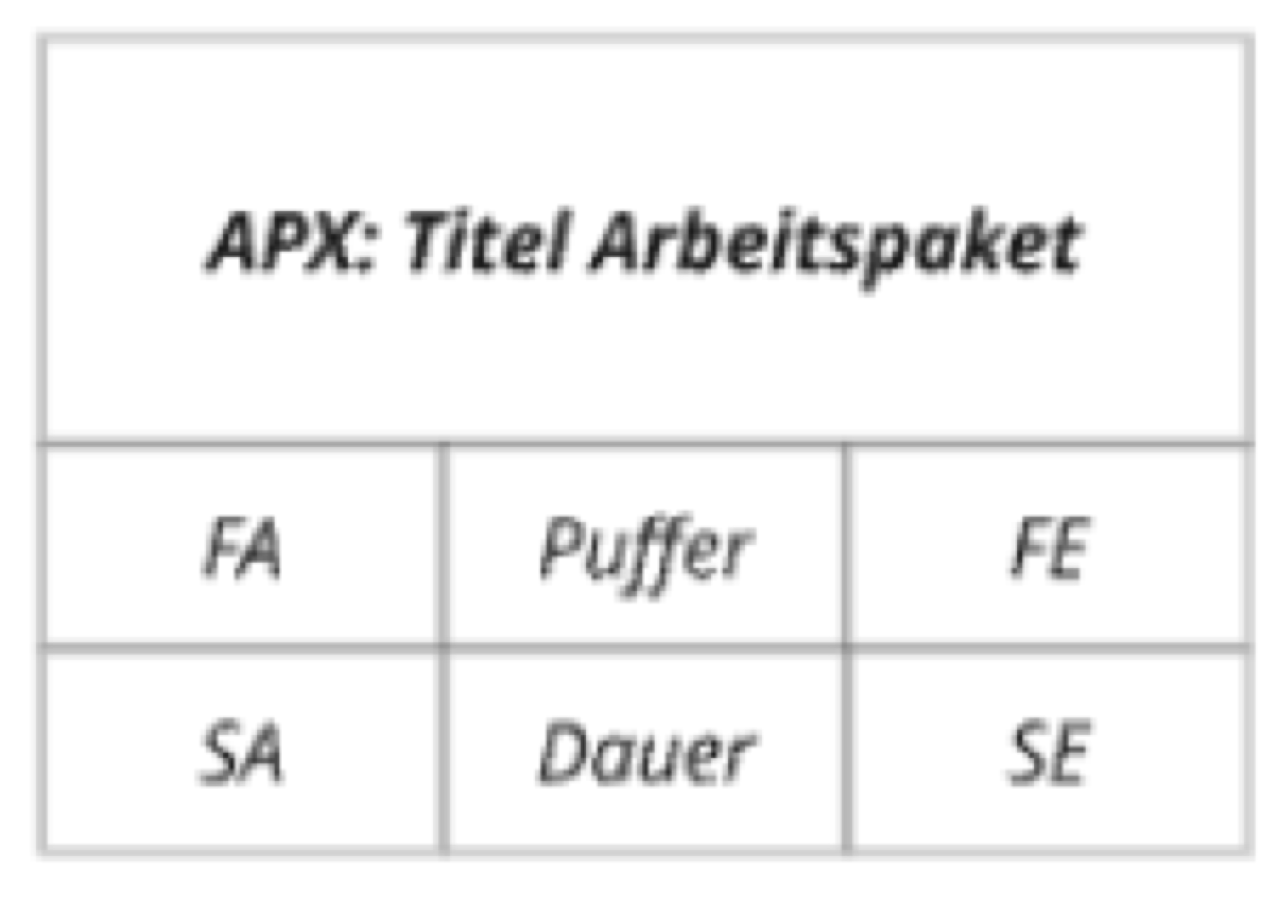
\includegraphics[width=0.15\textwidth]{fig/Netzplan info.png}
	\caption{Netzplan mit Markiertem Kritischen Pfad}
	\label{fig:netzplan}
\end{figure}
\pagebreak
%\section{Ressourcenzuordnung}
%Ressourcen werden zwei Hauptkategorien zugeordnet:

%\begin{itemize}
%  \item \textbf{Personalgruppen} - MA (z.B. Backend, DevOps, UX, QA)
%  \item \textbf{Sachmittel} - SM (z.B. Rechentechnik, Werkzeuge, Methoden)
%\end{itemize}
%Jedes Arbeitspaket hat einen gewissen bedarf an unterschiedlichen Gruppen und dieser wird ihnen zugeordnet.
%\\
%Eine detaillierte Zuordnung der Sachmittel erfolgte auf Ebene einzelner Arbeitspakete. Beispiele:
%\begin{itemize}
%  \item \textbf{AP1} – API-Gateway, Postman, CI-Tools
%  \item \textbf{AP5} – GPU-Server, NLP-Toolkits, Annotierungssoftware
%  \item \textbf{AP9} – IAM-Systeme, VPN, Sicherheits-Scanner
%\end{itemize}

\chapter{Terminplanung}
\label{sec:terminplanung}
\chapter{Kostenplanung}
\label{sec:kostenplanung}
\newpage
\newpage
\input{mainmatter/10_Qualitätssicherung.tex}
\chapter{Risikomanagement}
\label{sec:risikomanagement}

\section{ Risikoplanung}
Ziel der Risikoplanung ist es, potenzielle Gefahrenquellen im Projektverlauf frühzeitig zu erkennen, zu bewerten und geeignete Maßnahmen zur Risikovermeidung oder -Minderung zu definieren. Im Kontext unseres medizinischen Entity-Recognition-Systems sind insbesondere Qualität, Datenschutz, technische Integrität und Projektdurchlaufzeit zentrale Risikofaktoren, da sie direkte Auswirkungen auf Patientensicherheit, Klinikprozesse und regulatorische Vorhaben haben.
\section{Vorgehen}
Die Risikoplanung besteht nach ISO 31000 auf den folgenden Schritten:
\begin{enumerate}
	\item Identifikation potenzieller Risiken
	\item Kategorisierung und Bewertung nach Eintrittswahrscheinlichkeit und Schadenshöhe
	\item Ableitung geeigneter Gegenmaßnahmen
	\item Integration der Maßnahmen in die Projektplanung
	\item Laufende Überprüfung und Anpassung im Projektverlauf
\end{enumerate}
\section{Identifizierte Risiken und Bewertung}
\begin{center}
	\begin{tabular}{|p{4.5cm}|p{2.5cm}|p{2.5cm}|p{2.5cm}|p{3cm}|}
		\hline
		\textbf{Risiko} & \textbf{Eintritts- wahrscheinlichkeit} & \textbf{Schadens- ausmaß} & \textbf{Risikowert} & \textbf{Kategorie} \\
		\hline
		Verzögerung durch schlechte Datenqualität & Mittel & Hoch & Hoch & Datenmanagement \\
		\hline
		Unklare Anforderungen / Scope Creep & Hoch & Mittel & Hoch & Projektsteuerung \\
		\hline
		Ausfall von Schlüsselpersonen (Krankheit, Kündigung) & Mittel & Hoch & Hoch & Personalrisiko \\
		\hline
		Technologische Inkompatibilität (z.B. KI-Modelle <-> KIS-Systeme) & Niedrig & Hoch & Mittel & Technikrisiko \\
		\hline
		Sicherheitslücke / DSGVO-Verstoß bei Zugriffskontrolle & Niedrig bis Mittel & Sehr hoch & Hoch & Recht / Security \\
		\hline
		Unterfinanzierung durch falsch kalkulierte Betriebskosten & Niedrig & Hoch & Mittel & Finanzen \\
		\hline
		Zeitliche Engpässe in Test- und Abnahmephasen & Mittel & Mittel & Mittel & Qualität / Prozess \\
		\hline
	\end{tabular}
\end{center}
\section{Gegenmaßnahmen}
\begin{center}
	\begin{tabular}{|p{7cm}|p{9cm}|}
		\hline
		\textbf{Risiko} & \textbf{Geplante Gegenmaßnahme} \\
		\hline
		Schlechte Datenqualität & Validierung durch ETL-Tools, frühe Tests mit Musterdaten \\
		\hline
		Scope Creep / Anforderungsunsicherheit & Agile Methode mit Backlog-Pflege und Change Requests \\
		\hline
		Ausfall Schlüsselpersonen & Vertretungsregelung, Wissensdokumentation, Pair Programming \\
		\hline
		Inkompatible Technologien & Frühzeitige Prototypen, Schnittstellentests \\
		\hline
		DSGVO-Verstoß / Sicherheitslücke & Security-Audits, Datenschutzschulungen, automatisierte Tests \\
		\hline
		Falsche Kostenannahmen & Monatliche Kostenüberwachung, Kostenpuffer \\
		\hline
		Zeitengpässe in QS & QS kontinuierlich im Sprint, nicht nur zum Projektende \\
		\hline
	\end{tabular}
\end{center}

\newpage
\newpage

\input{mainmatter/11_Durchführungsplanung.tex}


\end{document}
